% @Author: Taha Bouhsine


%%%%%%%%%%%%%%%%%%%%%%%%%%%%
% CHAPTER                  %
%%%%%%%%%%%%%%%%%%%%%%%%%%%%
\setcounter{mtc}{12}

\chapter{Realization, GUI And Tests}%
\label{chap:chapter_four}
\minitoc

\section{Hardware Environments}

\subsection{Development hardware }
The good news is that you don’t need anything particularly special to run the development of mean stack. A single laptop or even a virtual machine \ac{VM} is enough to develop a MEAN application. All components of the stack can be installed on Windows, macOS, and most Linux distributions.

\subsection{Production hardware }
The approach to production hardware architecture isn’t all that different from development hardware. The main difference is that production hardware is normally higher-spec and open to the internet to receive public requests.

\begin{figure}[!ht]
      \centering
      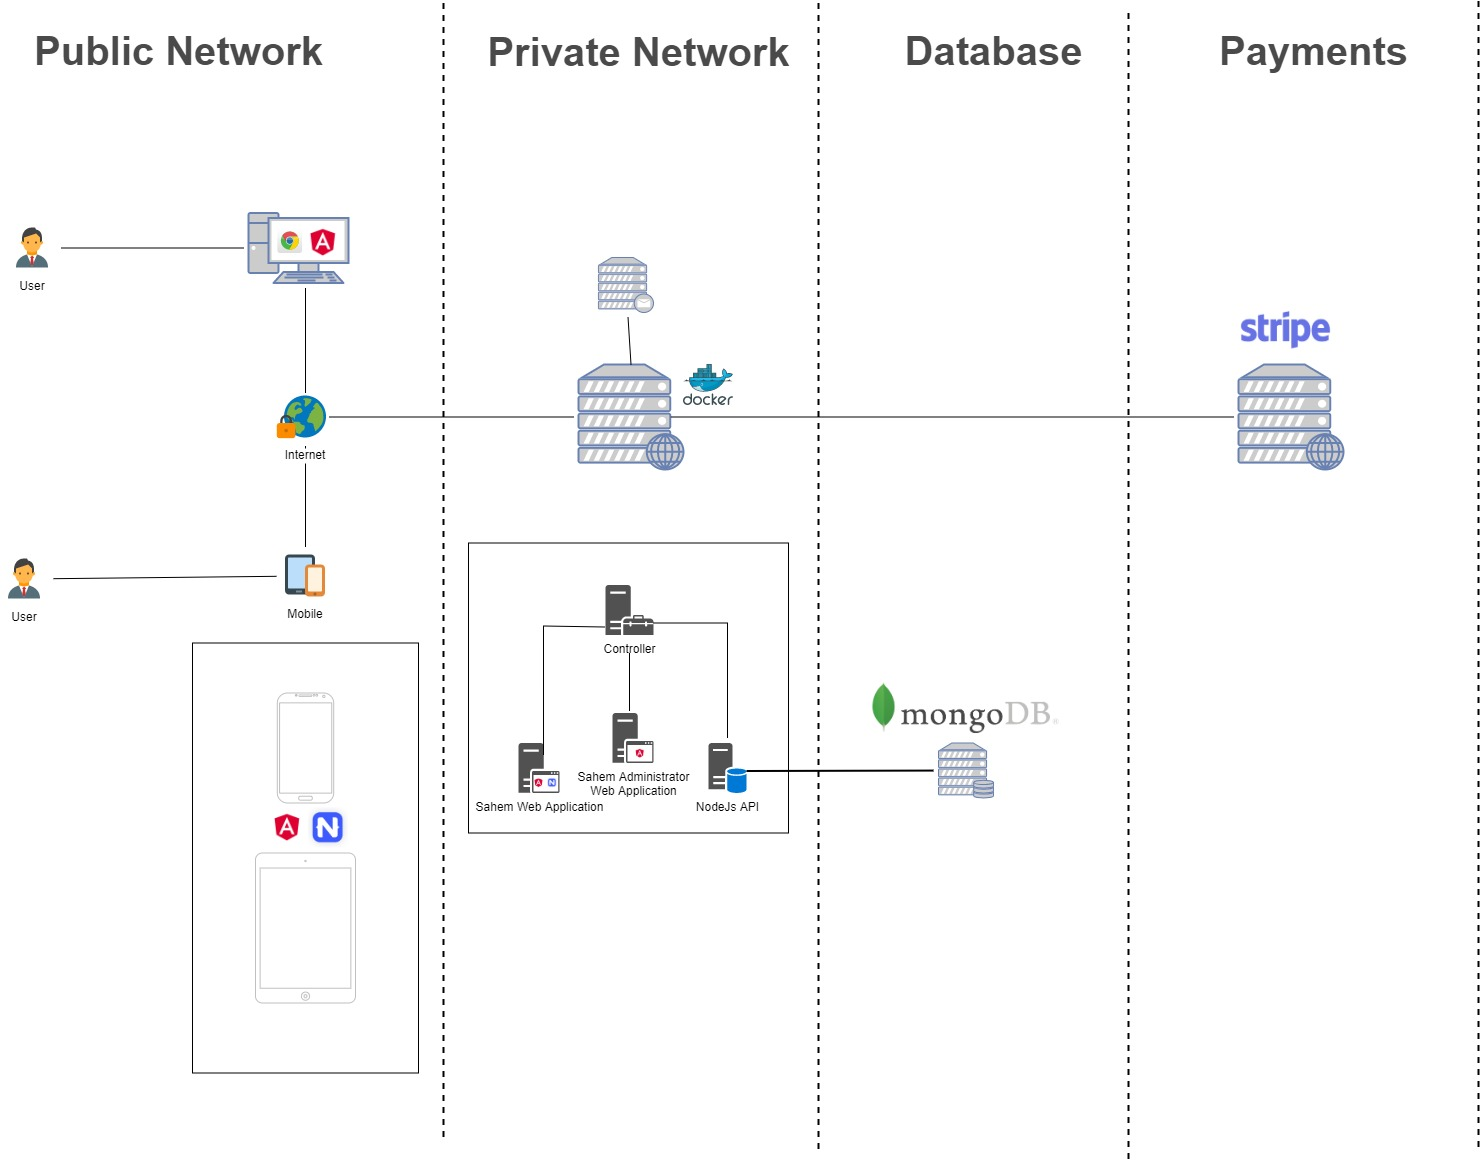
\includegraphics[scale=0.25]{assets/architecturedrawio.jpg}
      \caption{« Sahem » Platform's Hardware Architecture}
      \label{fig:sahemarchitecturedrawio}
\end{figure}
This model is commonly used when it comes to using \ac{PaaS} provider for hosting.
\section{Development Environments}
\subsection{Design And Planing}
In the modeling phase, we found many solutions and software that helped to create diagrams, but they all are graphic based solutions and felt a bit short. But we decided to work with the following tools.

\paragraph*{PlantUml}
PlantUML is an open-source tool allowing users to create UML diagrams from plain text language. The language of PlantUML is an example of a Domain-specific language. It uses Graphviz software to layout its diagrams. It has been used to allow blind students to work with UML. PlantUML also helps blind software engineers to design and read UML diagrams.

\paragraph*{Gantt chart}
A Gantt chart is a horizontal bar chart that visually represents a project plan over time. Modern Gantt charts typically show us the status of—as well as who’s responsible for—each task in the project.


\subsection{User Interface And Product Design}
\paragraph*{Adobe Photoshop}
Adobe Photoshop is a software application for image editing and photo retouching and logo creation. Photoshop offers users the ability to create, enhance, or otherwise edit images, artwork, and illustrations. It is the most widely used software tool for photo editing, image manipulation, and retouching for numerous image and video file formats.

\paragraph*{Adobe XD}
Adobe XD is a vector-based user experience design tool for web apps and mobile apps, developed and published by Adobe Inc. It is available for macOS and Windows, although there are versions for iOS and Android to help preview the result of work directly on mobile devices.



\subsection{Development}
\subsubsection{Version Control}
When building software it’s always important to track your changes. This is especially critical when collaborating on projects where multiple people will be updating the same code. Software that can keep track of all
these changes are called Version Control.

\paragraph*{Git}
% Git is a version control system for tracking changes in computer files and coordinating work on those files among multiple people. It is primarily used for source code management in software development, but it can be used to keep track of changes in any set of files. As a distributed revision control system it is aimed at speed, data integrity, and support for distributed, non-linear workflows.
Git is a distributed revision control and source code management system that
allows several people to work on the same codebase at the same time on different
computers and networks. These can be pushed together, with all changes stored and
recorded. It’s also possible to roll back to an earlier state if necessary.
\paragraph*{Github}
At a high level, GitHub is a website and cloud-based service that helps developers store and manage their code, as well as track and control changes to their code.

\paragraph*{Github Desktop}
GitHub Desktop is a fast and easy way to contribute to projects, and is designed to simplify all processes and workflow in our GitHub.

\subsubsection{Dependency Managers}
A large software project often makes use of many third-party packages and libraries. In turn, these packages
often rely on several other packages and so on. To keep track of all these dependencies, software developers
use-package managers. Below we introduce the ones we have used.
\paragraph*{Node Package Manager}
Node Package Manager \ac{NPM}, is two things: first and foremost, it is an online repository for the publishing of open-source Node.js projects; second, it is a command-line utility for interacting with the said repository that aids in package installation, version management, and dependency management.
\paragraph*{Angular CLI}
The Angular CLI is a command-line interface tool that we use to initialize, develop, scaffold, and maintain Angular applications. 
\subsubsection{IDEs}

\paragraph*{Visual Studio Code}
Visual Studio Code is a source code editor developed by Microsoft for Windows, Linux, and macOS. It includes support for debugging, embedded Git control and GitHub, syntax highlighting, intelligent code completion, snippets, and code refactoring.


\paragraph*{MongoDB Compass Community}
MongoDB Compass is the defacto GUI tool for MongoDB much like MySQL Workbench is MySQL’s associated tool. It allows us to visually explore our data, run ad hoc queries, interact with our data with full CRUD functionality, as well as view and optimize our queries’ performance.


\paragraph*{Postman}
Postman is an interactive and automatic tool for verifying the APIs of our project. Postman is a Google Chrome app for interacting with HTTP APIs. It presents us with a friendly GUI for constructing requests and reading responses. It works on the backend, and makes sure that each API is working as intended.




\subsubsection{Report And Presentation}
\paragraph*{Boost Note}
Boostnote is an Open source note-taking app for programmers.

\paragraph*{Latex}
\latex{} is a tool used to create professional-looking documents. It is based on the WYSIWYM (what we see is what we mean) idea, meaning we only have to focus on the contents of our document and the computer will take care of the formatting. Instead of spacing out text on a page to control formatting, as with Microsoft Word or LibreOffice Writer, users can enter plain text and let LATEX take care of the rest.
% \paragraph*{MiKTex}
% MiKTeX provides the tools necessary to prepare documents using the TeX/LaTeX markup language, as well as a simple tex editor: TeXworks.

% \paragraph*{Tex Live}
% TeX Live is intended to be a straightforward way to get up and running with the TeX document production system. It provides a comprehensive TeX system with binaries for most flavors of Unix, including GNU/Linux, macOS, and also Windows. It includes all the major TeX-related programs, macro packages, and fonts that are free software, including support for many languages around the world. Many operating systems provide it via their distributions.



\paragraph*{Markdown}
Markdown is a lightweight markup language with plain-text-formatting syntax. Its design allows it to be converted to many output formats, but the original tool by the same name only supports HTML. Markdown is often used to format readme files, for writing messages in online discussion forums, and to create rich text using a plain text editor.

\paragraph*{Marp}
Marp is the ecosystem to write our presentation with plain Markdown.


% section
% section
% section
\section{Platform security}
Security is a constant worry when it comes to information technology. Data theft, hacking, malware, and a host of other threats are enough to keep any IT professional up at night. In this article, we’ll look at the basic principles and best practices that IT professionals use to keep their systems safe.

When you create a website or application, it means you are ready to show thousands of people on the internet. Your customer/audience may be legit, but some of them will try to tamper your application. So we need to follow the following golden rules:
\begin{enumerate}
      \item 
      “Never trust your audience when it comes to your application’s security”
      \item 
      Always validate the user input before getting it into the server.
      \item 
      Always encode the user inputs before printing them on to the screen.
\end{enumerate}

\subsection{Security Principles}
The main three overarching principles in information security are:
\begin{enumerate}
      \item 
      Confidentiality: This means that information is only being seen or used by people who are authorized to access it.
      \item 
      Integrity: This means that any changes to the information by an unauthorized user are impossible (or at least detected), and changes by authorized users are tracked.
      \item 
      Availability: This means that the information is accessible when authorized users need it.
\end{enumerate}

\subsection{Physical level}
For the Physical level, we will be hosting and deploying our application to an IaaS cloud service, the main reason to use the cloud services is the ability they provide to our application to be decentralized, and available all time.

Physical security on IaaS is managed by one or several processes, which include:
\begin{enumerate}
      \item 
      Area security definition
      \item 
      Controlled access to those areas
      \item 
      Uninterrupted power supplies
      \item 
      Monitoring critical parameters
      \item 
      Alarms
      \item 
      Air and particle filtering
      \item 
      Fire protection
      \item 
      Others, such as proper risk and issue management
\end{enumerate}
\subsection{Logical level}
Logical Security consists of software safeguards for an organization's systems, including user identification and password access, authenticating, access rights, and authority levels. These measures are to ensure that only authorized users are able to perform actions or access information in a network or a workstation.
We have implemented multiple levels and layers of security to control the integrity of the data exchanged between our users and « Sahem » platform, from creating form controls to ensure that the data sent from the user is well structured, and when received on the controller, we created multiple layers and implemented some great middlewares and libraries to help us protect the system from different vulnerabilities.

And for the Confidentiality, on the Frontend we put guards on our routes, to only give some specific users the accessibility to the functionalities they have the permission to do, and when a request is received on the controller, we check the user's Identity, and check if they are allowed to take the action requested.
\subsubsection{Stripe Payment API}
Stripe was founded in 2010 with the mission of making it easier to accept payments over the internet. At the time, taking credit cards meant working with a legacy processor or a middleman broker who would provide you with access to a processor.
Stripe has been audited by a PCI-certified auditor and is certified to PCI Service Provider Level 1. This is the most stringent level of certification available in the payments industry.

They use the best-in-class security tools and practices to maintain a high level of security at Stripe:
\begin{enumerate}
      \item HTTPS and HSTS for secure connections
      \item Encryption of sensitive data and communication
      \item PGP keys to encrypt your communications with Stripe
\end{enumerate}
\subsubsection{Frontend}
Angular has some great protections against common web-application vulnerabilities and attacks to provide it's applications with a good, and secure experience, preventing cross-site scripting \ac{XSS} that prevent attackers from injecting malicious code into web pages. Such code can then, for example, steal user data (in particular, login data) or perform actions to impersonate the user. This is one of the most common attacks on the web.

And has built-in support to help prevent two common HTTP vulnerabilities, cross-site request forgery (\ac{CSRF} or XSRF) and cross-site script inclusion \ac{XSSI}. Both of these must be mitigated primarily on the server-side, but Angular provides helpers to make integration on the client-side easier.

\paragraph*{Route Guards}
Angular’s route guards are interfaces that can tell the router whether or not it should allow navigation to a requested route. They make this decision by looking for a true or false return value from a class that implements the given guard interface.
\paragraph*{Form Control}
This is one of the three fundamental building blocks of Angular. It implements most of the base functionality for accessing the value, validation status, user interactions, and events.
\subsubsection{BackEnd}
Security is really hard to get right on the backend. There are so many different factors to consider, countless different ways to break an application. 
This is just as true with Express applications as it is with any other web framework. There's no instant way to make sure an application won't be taken down by a Denial of Service (DoS) attack because of how it handles one type of user input, or how it routes a specific request.
\paragraph*{Error Handling}
Error handling is considered one of the main factors in creating a good production software for any type of applications, so we have made it our main 
\paragraph*{Check for Vulnerabilities}
There are a few tools in the Node ecosystem that allow easy checking for vulnerabilities in Node and Express application dependencies. These tools are highly valuable in ensuring that no vulnerabilities are currently in the packages an application relies on, and none are added into that application when its packages are updated.
\begin{enumerate}
      \item Snyk
      \item Node Security Project
      \item Retire.js
\end{enumerate}

\paragraph*{Helmet}
\paragraph*{HTTP headers}
The helmet middleware is really like a helmet for our applications. It protects our application by setting up various HTTP headers.
\paragraph*{Session Date}
The express-session middleware stores session data on the server; it only saves the session ID in the cookie itself, not session data.

\paragraph*{cookie-session}
Cookie-session is a simple cookie-based session middleware, that allows storing cookies.It doesn't require any database/resources on the server-side, though the total session data cannot exceed the browser’s max cookie size.

\paragraph*{Authentication}
express-jwt-permissions is a middleware that checks \ac{JWT} tokens for permissions. It is very useful to build a user access control system.

\paragraph*{Data sanitize}
Express-mongo-sanitize is a middleware that sanitizes user-supplied data to prevent MongoDB Operator Injection.

\paragraph*{Errors Logging}
Morgan is a library adds some logging capabilities to our Express API.

\paragraph*{Cross-Origin Resource Sharing}
We will use Cors dependency to configure Express to add headers stating that your API accepts requests coming from other origins. This is known as Cross-Origin Resource Sharing \ac{CORS}.
\paragraph*{Server's Information}
Dotenv is a zero-dependency module that loads environment variables from a .env file into process.env.. Storing configuration in the environment separate from code is based on The Twelve-Factor App methodology \cite{web004}.





\section{Project Tests}
Project testing and validation is the last step of the software engineering process. The
Testing is conducted during or after the implementation in order to ascertain that the product is
compliant with the requirements and modeling specifications initially stipulated in the
analysis and design phase, i.e. whether or not the product, « Sahem » Crowdfunding Platform
in our case, satisfies and meets the needs, requirements, and design initially stipulated.
The testing process for our application comprised of Unite testing through Jasmine and Karma for
the angular application, and Mockgoose for our express js controller, then use Protractor.js to perform
end to end testing.
This is achieved by test targeting specific and small portions of code such as individual classes or
functions. 
The Integration Testing is done by verifying and testing the interaction between the
different components of our app as they were integrated in addition to the data flow between
them.
 Many errors and system failures occurred during this step and are being dealt
with. Concerning System Testing, this is conducted by testing the system as a whole to ensure
that the requirements, both functional and non-functional are met. The final step of the testing
phase, which represents the Acceptance Testing will be conducted by \mentor to see whether the project
meets the requirements stated earlier or not.
% Karma for angular
% Mockgoose for mongoose
% Protractor.js end to end testing

% section

\section{Deployment}
% section
% 
Today, there exist multiple PaaS on the internet, that gives a lot of rich environments with NodeJs
included. Sadly, most of them are paid, and those that provide the free tier services, puts a lot
of constraints on the application, such as Heroku, that we will be using to deploy our application,
it does delete all the static files on every server restart, and shuts down the server when it does
not receive any request for some time. But one of the positive points was that we could deploy the
application by linking it to the development repository on Github.


\url{https://sahem.herokuapp.com/}

% heroku free tier 

\section{Interfaces}
% section
% section
% section

One of the main requirements for our Frontend application was to create a responsive design to fit our
application in different devices and screen sizes. 

\begin{figure}[H]
      \centering
      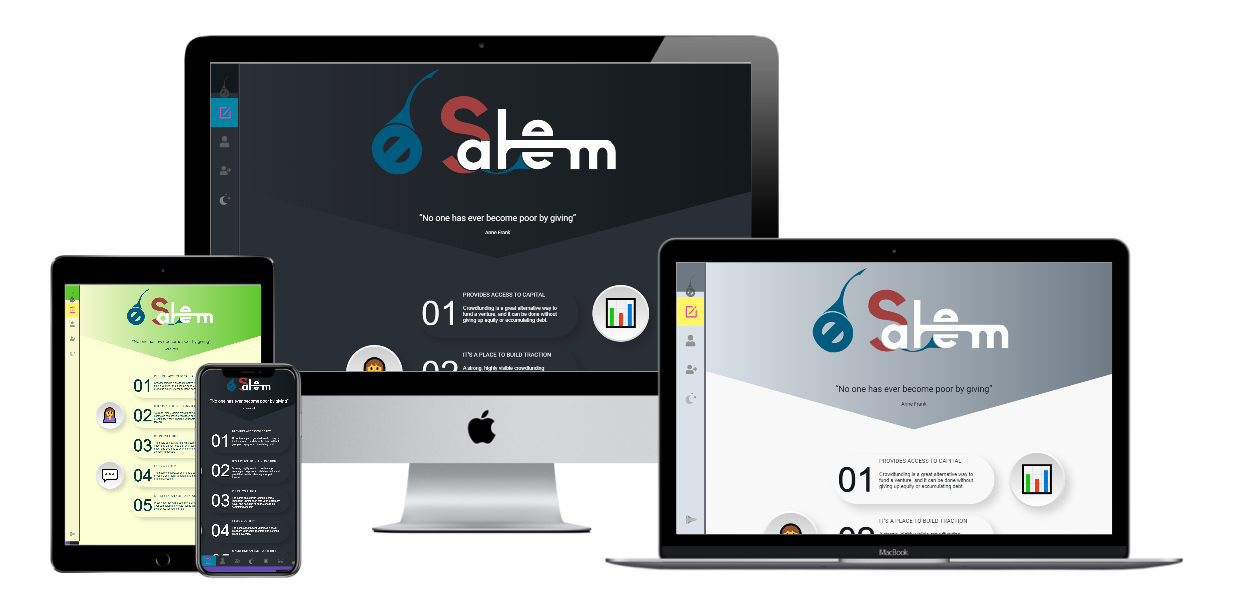
\includegraphics[scale=0.45]{assets/allDevices.png}
      \caption{Responsive Design}
      \label{fig:all devices}
\end{figure}

%%%%%%%%%%%% main %%%%%%%%

\begin{figure}[H]
      \centering
      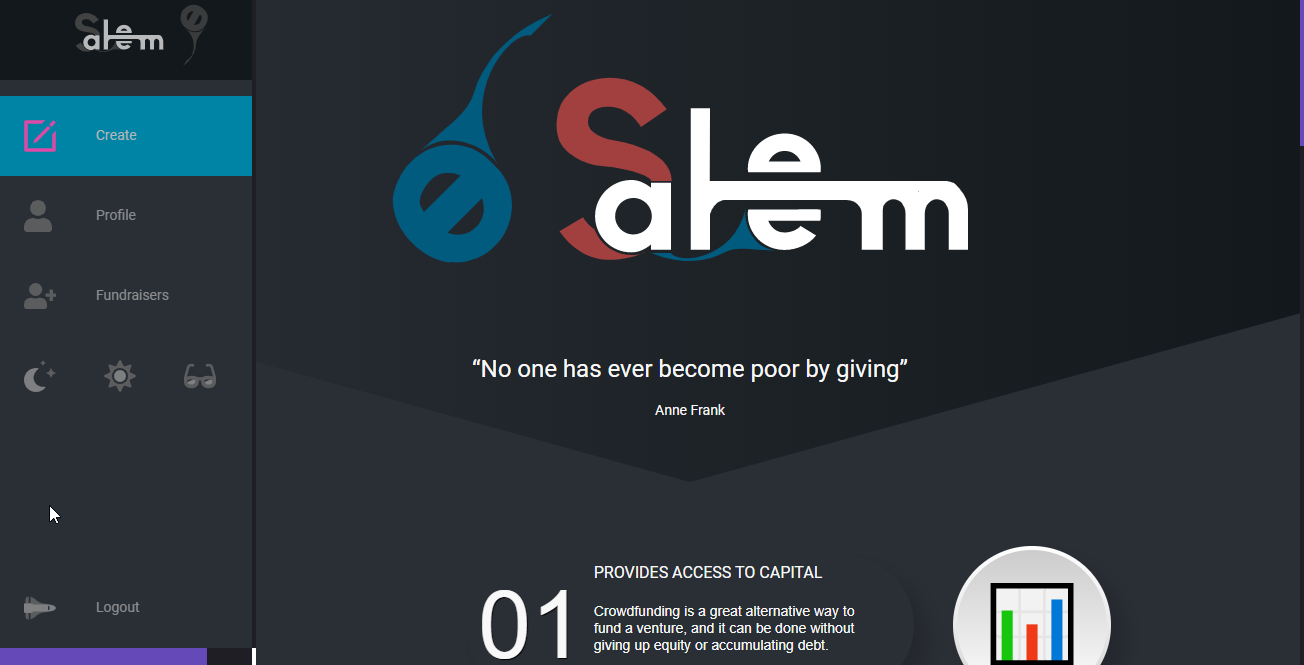
\includegraphics[scale=0.45]{assets/screen-main-navbar.png}
      \caption{« Sahem » Main Page - Navbar Activated}
      \label{fig:sahem main}
\end{figure}

The application comes with different themes and colors to satisfy multiple varieties of users.
\begin{figure}
      \centering
      \begin{subfigure}[H]{0.45\textwidth}
          \centering
          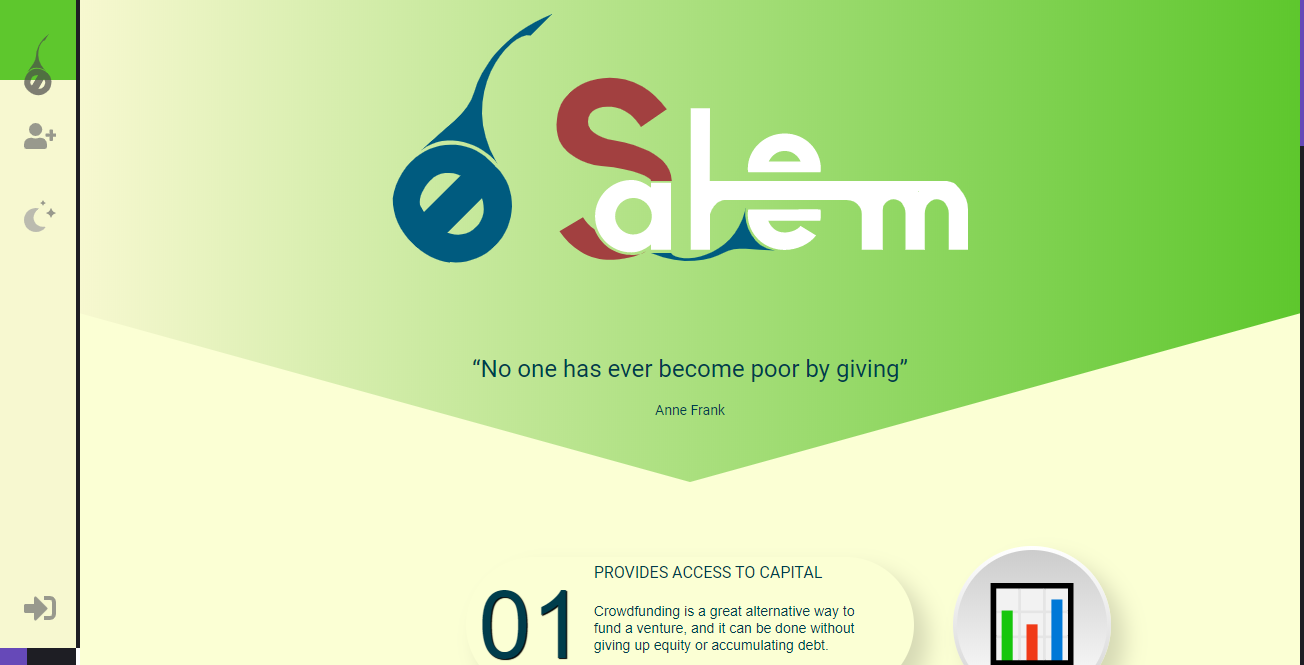
\includegraphics[width=\textwidth]{assets/screen-main-gre.png}
      \end{subfigure}
      \hfill
      \begin{subfigure}[H]{0.45\textwidth}
          \centering
          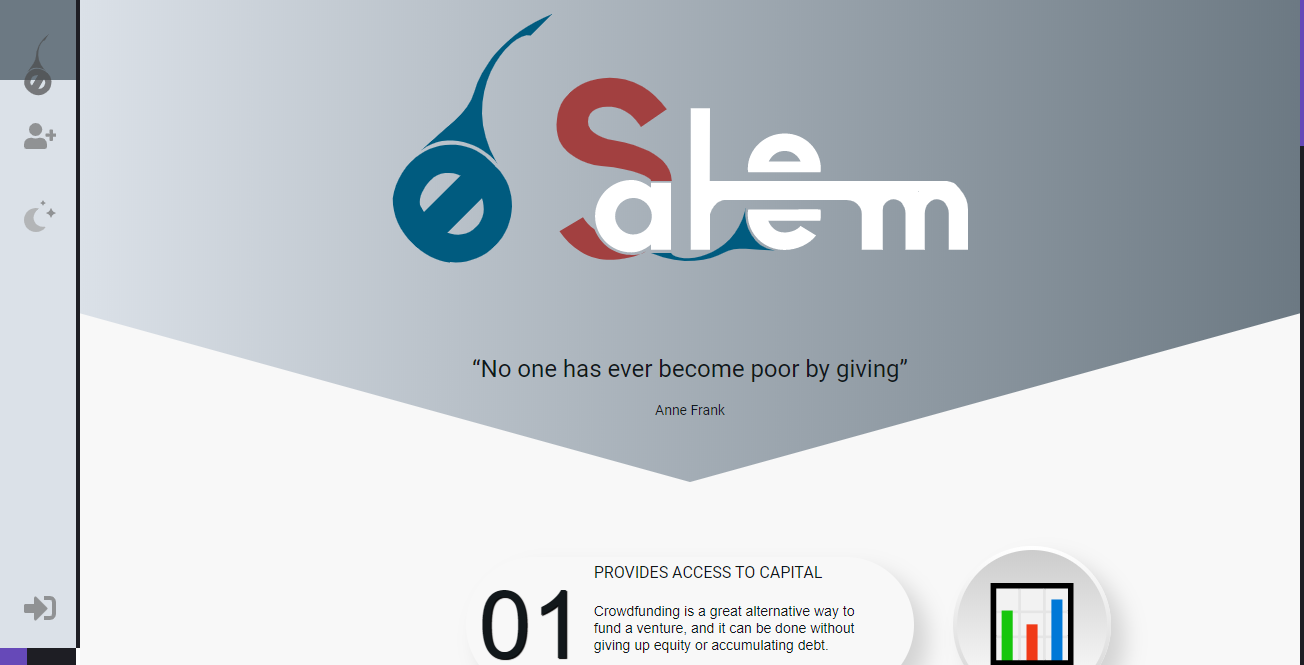
\includegraphics[width=\textwidth]{assets/screen-main-grey.png}
      \end{subfigure}
      \caption{« Sahem » Main Page - Themes}
      
 \end{figure}

 \begin{figure}[H]
      \centering
      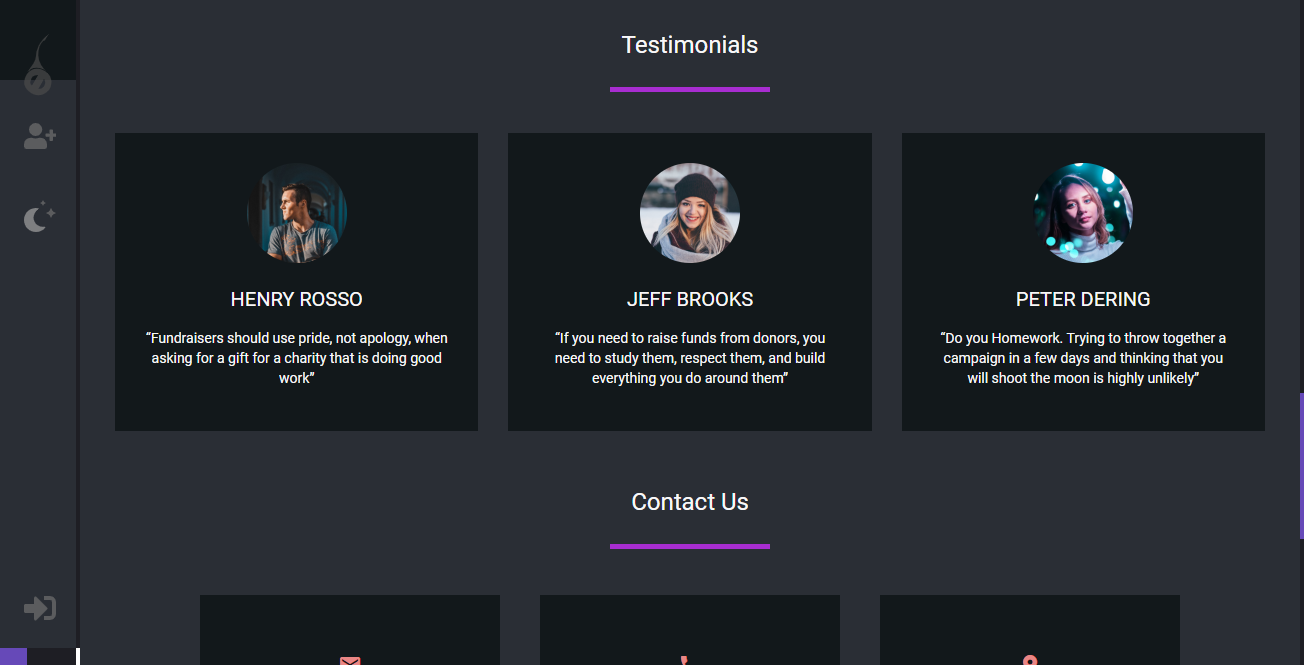
\includegraphics[scale=0.45]{assets/screen-main-test.png}
      \caption{« Sahem » Main Page - Testimonials}

      \label{fig:testimonials}
\end{figure}
\begin{figure}[H]
      \centering
      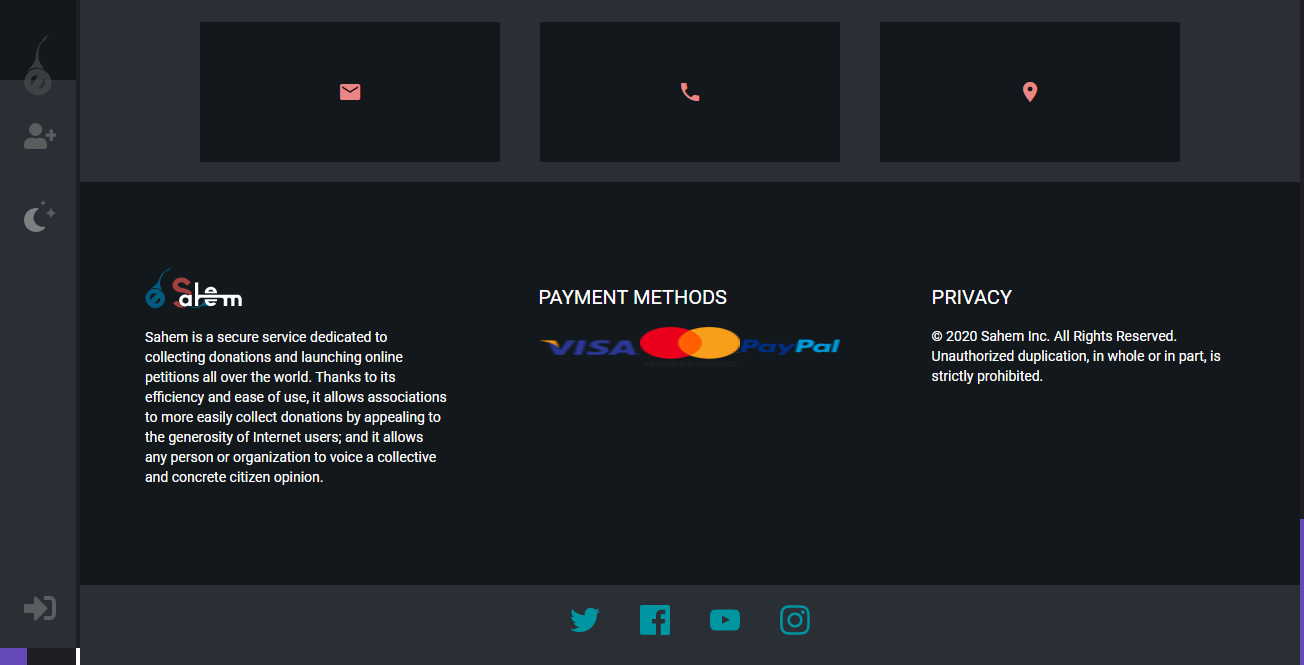
\includegraphics[scale=0.45]{assets/screen-main-foot.png}
      \caption{« Sahem » Main Page - Footer}

      \label{fig:footer}
\end{figure}






%%%%%%%%%%%%%%%%%% login register
The Angular framework provides us with a rich form control experience. With it, we designed and created multiple delicate forms Figure~\ref{fig:login page} and Figure~\ref{fig:register page}. 
\begin{figure}[H]
      \centering
      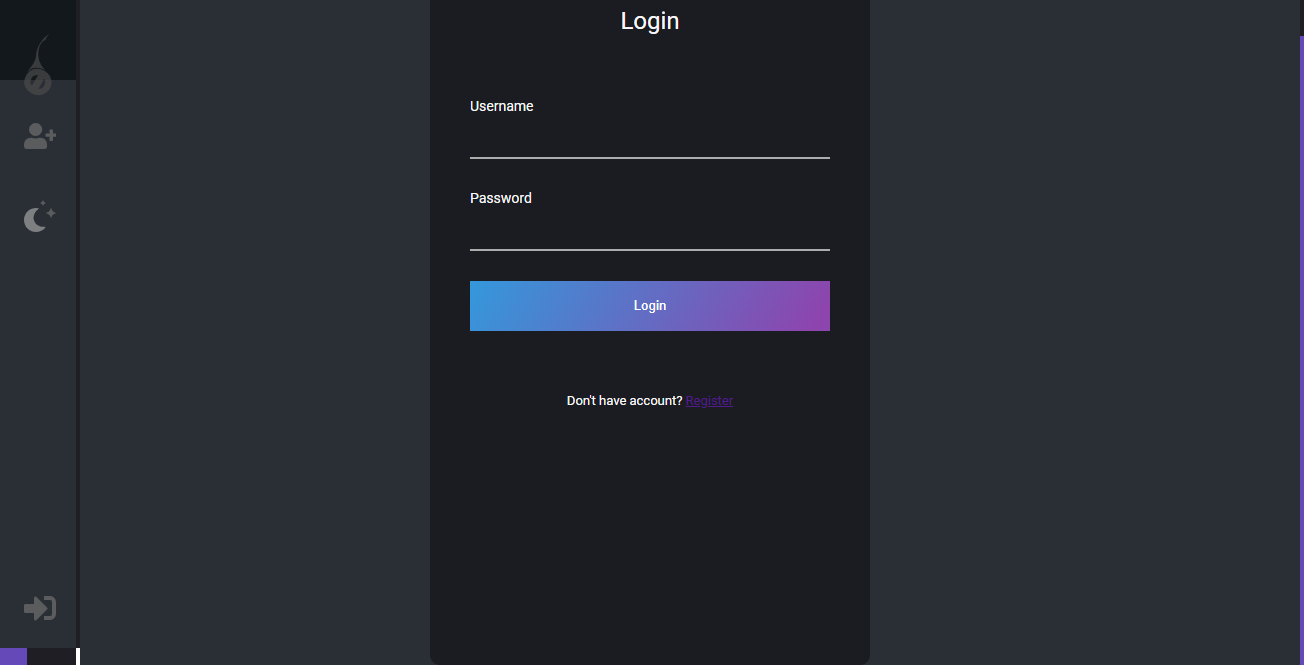
\includegraphics[scale=0.45]{assets/screen-login.png}
      \caption{Login Page}
      \label{fig:login page}
\end{figure}

\begin{figure}
      \centering
      \begin{subfigure}[H]{0.4\textwidth}
          \centering
          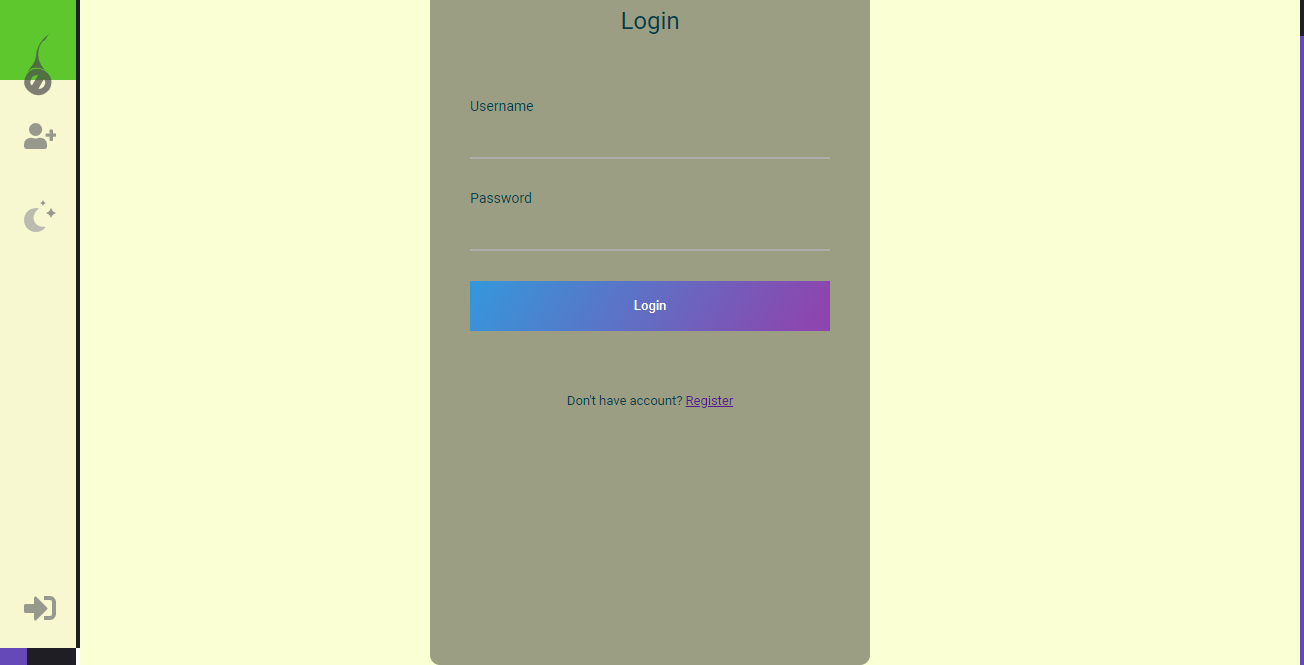
\includegraphics[width=\textwidth]{assets/screen-login-gr.png}
      \end{subfigure}
      \hfill
      \begin{subfigure}[H]{0.4\textwidth}
          \centering
          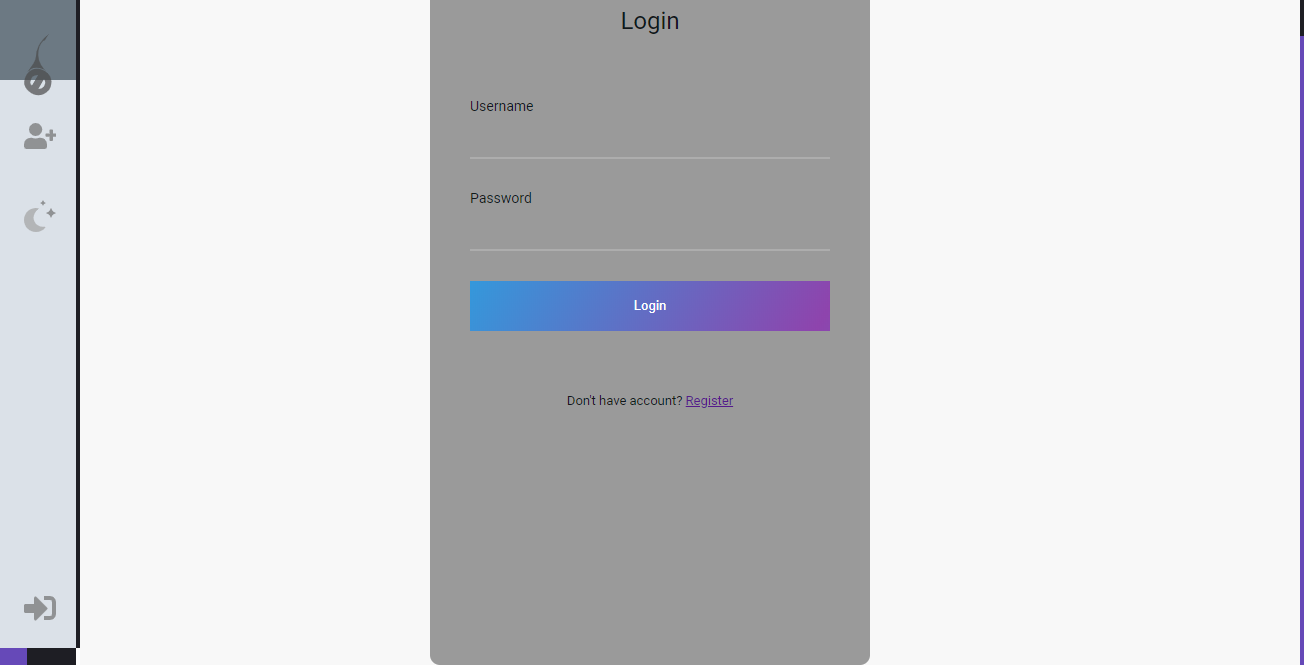
\includegraphics[width=\textwidth]{assets/screen-login-grey.png}
      \end{subfigure}
      \caption{Login Page - Themes}
      
 \end{figure}



% register


\begin{figure}[H]
      \centering
      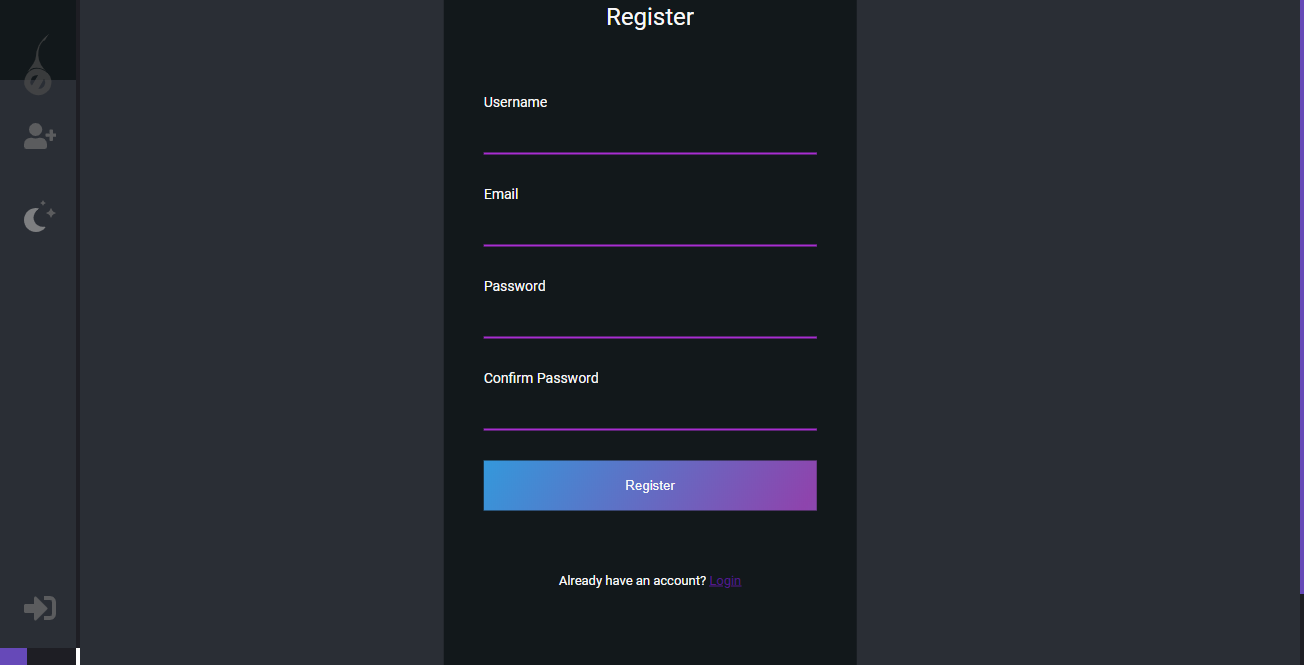
\includegraphics[scale=0.45]{assets/screen-register-d.png}
      \caption{Register Page}
      \label{fig:register page}
\end{figure}

%%%%%%%%%%%%%%%% create

Figure~\ref{fig:fundraiser form} is a form that allows the user to create a fundraiser.

\begin{figure}[H]
      \centering
      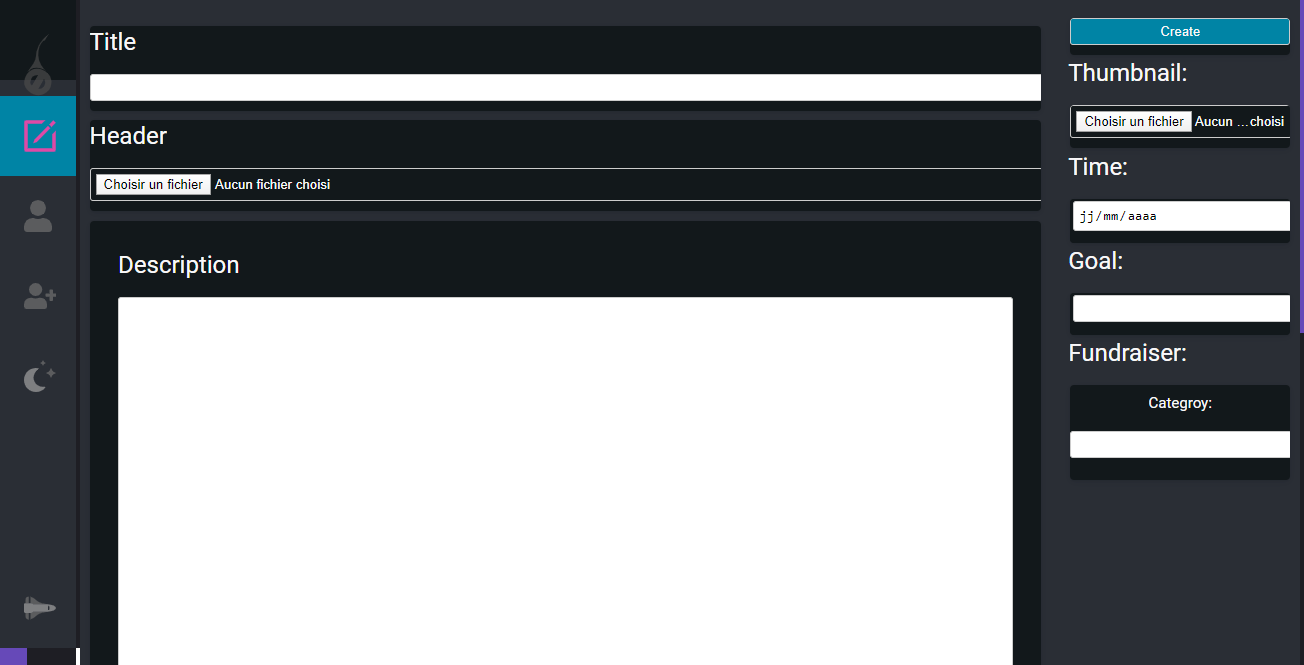
\includegraphics[scale=0.45]{assets/screen-fundraiser-creator.png}
      \caption{Fundraiser Form}
      \label{fig:fundraiser form}
\end{figure}


%%%%%%%%%%%%%%%%%%%% fundraisers

Figure~\ref{fig:fundraisers list} is a showcase with the in-progress projects existing on the platform.
\begin{figure}[H]
      \centering
      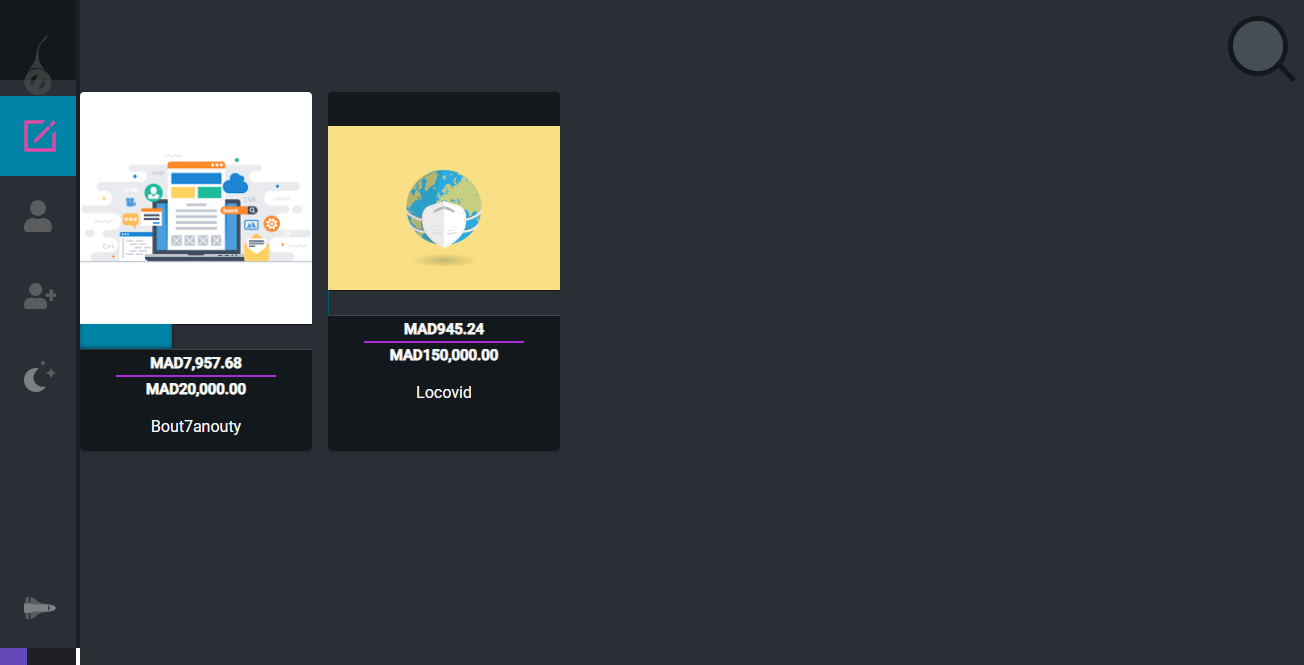
\includegraphics[scale=0.45]{assets/screen-fundraisers-list.png}
      \caption{Fundraisers List}
      \label{fig:fundraisers list}
\end{figure}



%%%%%%%%%%%%%%%%%%% fundraiser

Figure~\ref{fig:fundraiser view} is an example of the content of a created fundraiser.
\begin{figure}[H]
      \centering
      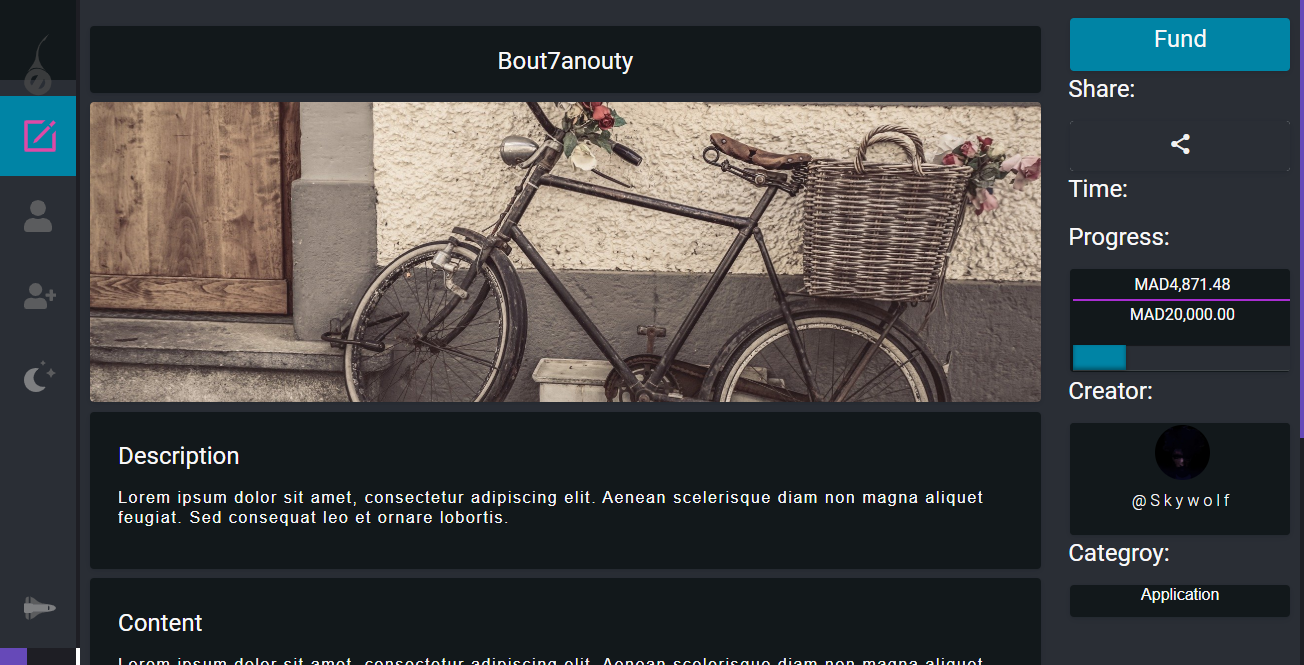
\includegraphics[scale=0.45]{assets/screen-fundraiser-view.png}
      \caption{Fundraiser View}
      \label{fig:fundraiser view}
\end{figure}



%%%%%%%%%%%%%%%%%%% profile
% profile create
When a user accesses his profile for the first time, he will be asked to fill the form in Figure~\ref{fig:profile form} 
to create his Profile, he won't be able to create a fundraiser otherwise.

\begin{figure}[H]
      \centering
      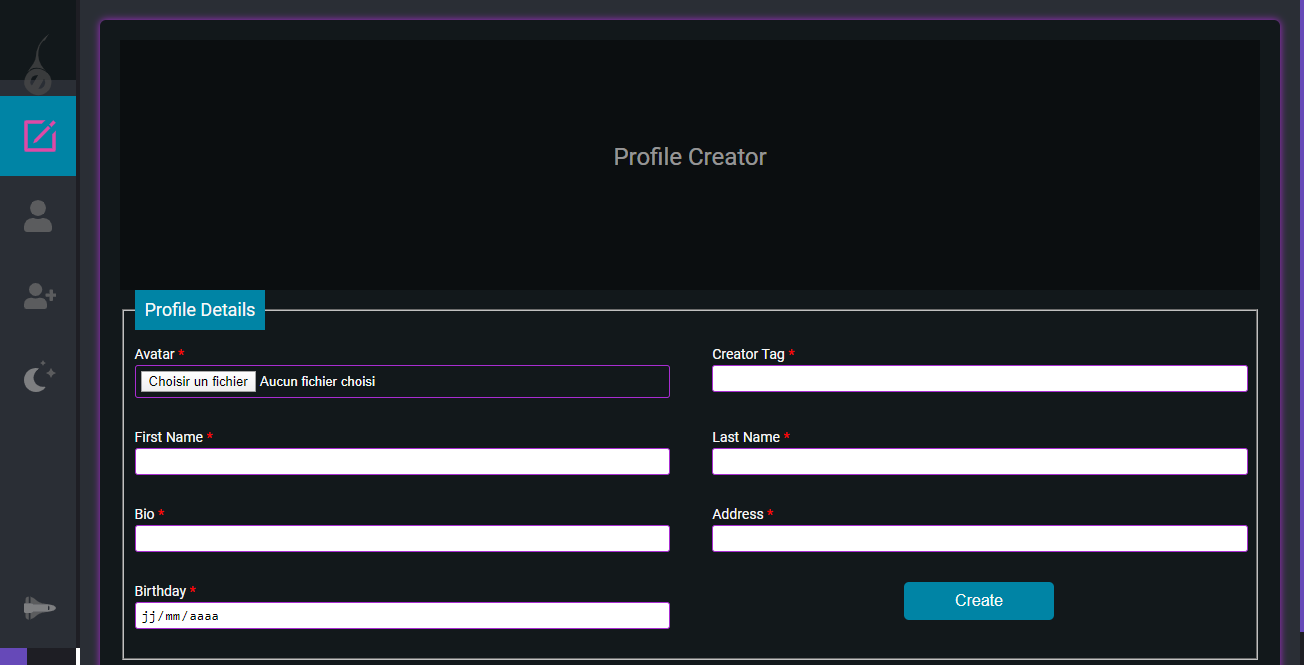
\includegraphics[scale=0.45]{assets/screen-profile-creator.png}
      \caption{Profile Form}
      \label{fig:profile form}
\end{figure}

% profile view
For every user there exist a profile that holds his information, Figure~\ref{fig:profile view} is page showcase the different fundraisers 
he created and successfully funded.
\begin{figure}[H]
      \centering
      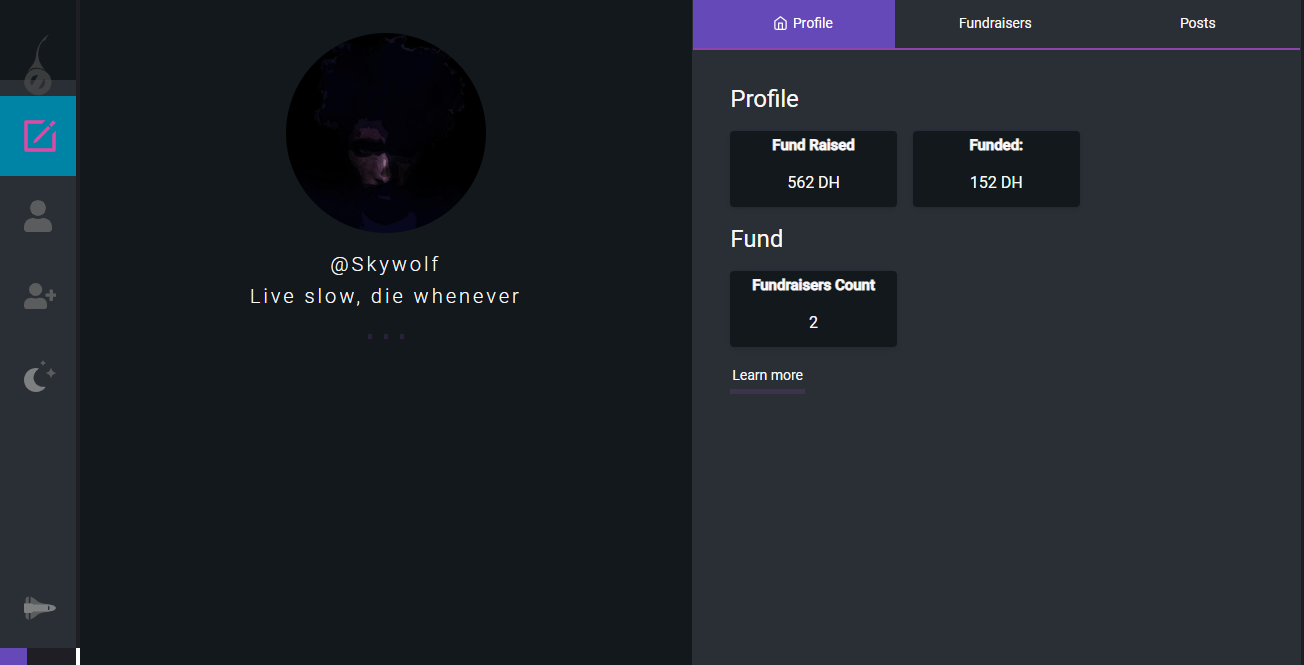
\includegraphics[scale=0.45]{assets/screen-profile-da.png}
      \caption{Profile Page}
      \label{fig:profile view}
\end{figure}

\begin{figure}
      \centering
      \begin{subfigure}[H]{0.4\textwidth}
          \centering
          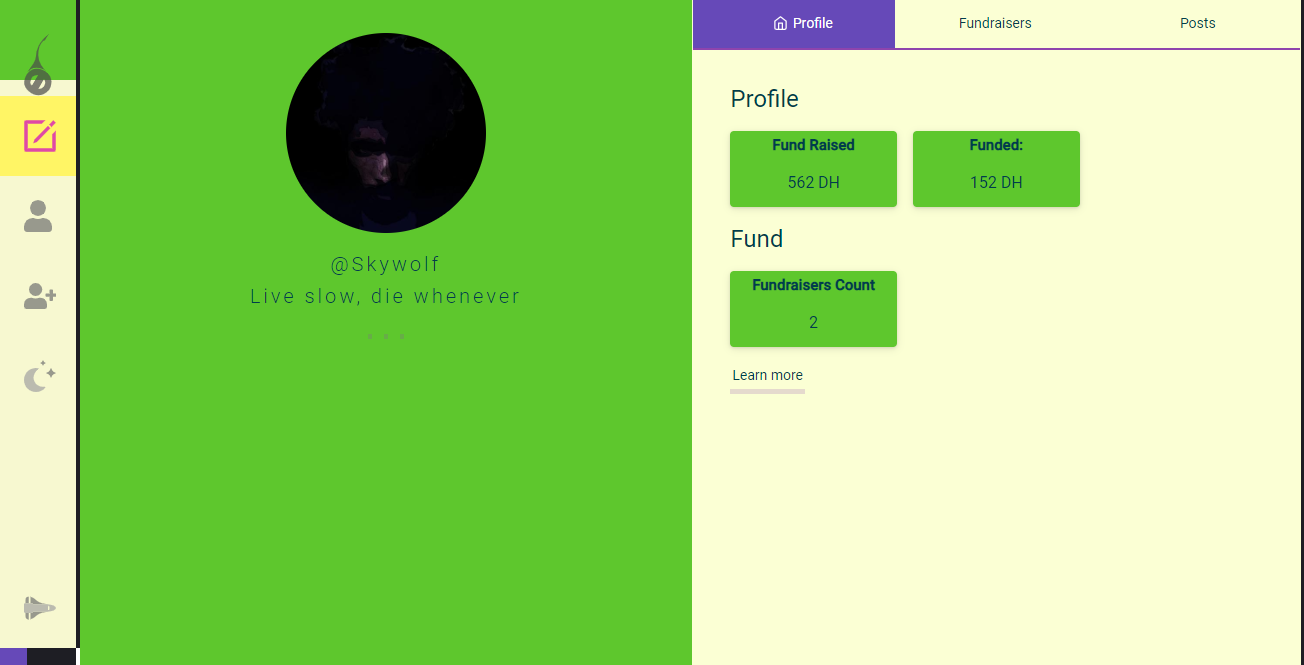
\includegraphics[width=\textwidth]{assets/screen-profile-gre.png}
      \end{subfigure}
      \hfill
      \begin{subfigure}[H]{0.4\textwidth}
          \centering
          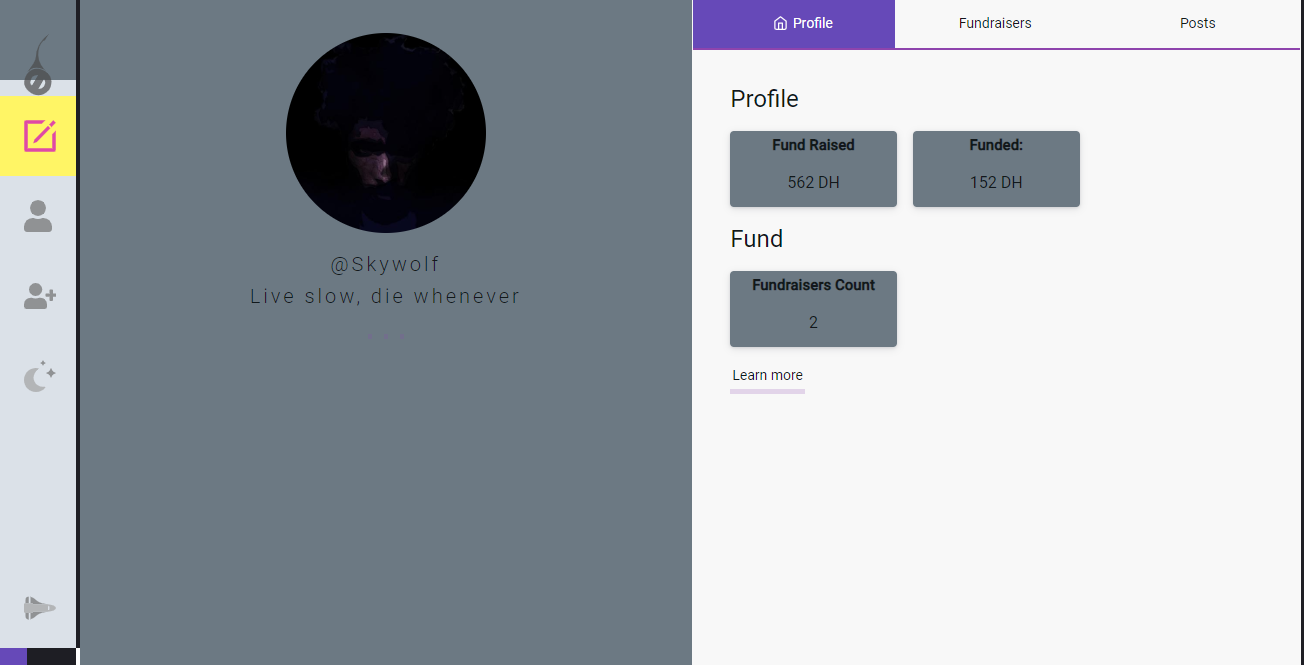
\includegraphics[width=\textwidth]{assets/screen-profile-grey.png}
      \end{subfigure}
      \caption{Profile Page - Themes}
  
 \end{figure}



% section
% section
% section
% section


